\chapter{Grundlagen und Verwandte Arbeiten}

Dieses Kapitel beschreibt verwandte Arbeiten und die Grundlagen von Erklärbarkeit sowie dessen Zusammenwirkung mit zusammenhängenden NFRs.

\section{Erklärungen in erklärbaren Systemen}
\label{02_basics:explainable_system}

Erklärungen in erklärbaren Systemen werden unter dem Oberbegriff Erklärbarkeit (\textit{Explainability}) zusammengefasst. Darunter wird das Integrieren von Erklärungen in erklärbare Systeme und die damit verbundenen Auswirkungen auf die Softwarequalität untersucht. Der Aspekt wird von unterschiedlichen Autoren durch verschiedene Synonyme beschrieben. \citeauthor{brennen_what_2020} hat einen Katalog zusammengestellt, welcher einige Synonyme zusammenfasst \cite{brennen_what_2020}. Dieser enthält unter anderem die Begriffe
% \textit{Accountability}, \textit{Trust}, 
\textit{Transparency}, \textit{Understandability} und \textit{Interpretability}. In der jüngeren Vergangenheit haben verschiedene Autoren diese Begriffe mit differenzierten Bedeutungen in einen Zusammenhang mit \textit{Explainability} gestellt \cite{chazette_end-users_nodate,chazette_knowledge_nodate,kohl_explainability_2019,wang_integration_2020}.

\textit{Transparency} wird als der Grad, zu dem ein System Einblick in dessen Funktionsweise gewährt, beschrieben \cite{chazette_end-users_nodate}. Diese Offenlegung kann dabei verschiedene Aspekte von Systemen wie zugrundeliegende Algorithmen z.~B. in Empfehlungssystemen \cite{balog_measuring_2020} oder trainierte Modelle des Maschinellen Lernens \cite{sovrano_modelling_2020} betreffen.

Das Verstehen von Erklärungen wird unter \textit{Understandability} zusammengefasst \cite{do2010software}. Das so erlangte Verständnis von Systemnutzern ist folglich als subjektiver Einflussfaktor für Erklärungen zu werten \cite{chazette_end-users_nodate}. Für diesen subjektiven Faktor nutzen \citeauthor{wang_integration_2020} sowie \citeauthor{balog_measuring_2020} den Begriff \textit{Perceived Transparency} als Synonym, um die subjektive Aufnahme von \textit{Transparency} bei verschiedenem Verständnis durch Nutzer zu verdeutlichen \cite{wang_integration_2020, balog_measuring_2020}.

Während \textit{Interpretability} zum Teil mit \textit{Understandability} gleichgesetzt wird \cite{chazette_end-users_nodate}, nimmt die Verwendung des Begriffs für den Grad der möglichen Interpretation der Ausgaben von ML-Algorithmen zu \cite{doshi2017towards}. Als Abgrenzung zwischen \textit{Explainability} und \textit{Interpretability} wird ersteres dabei auch als \glqq Top-Down\grqq{}-Verständnis und letzteres als \glqq Bottom-up\grqq{}-Verständnis beschrieben \cite{thomson_knowledge--information_2020}.

Da der Fokus dieser Arbeit auf externen Qualitätsaspekten liegt, ist die \textit{Interpretability} von ML-Algorithmen kein Bestandteil dieser Arbeit. Um trotz dessen einer Irritation durch doppelt belegte Begriffe vorzubeugen, wird für den subjektiven Faktor des Verständnisses von Softwaresystem \textit{Perceived Transparency} verwendet.

\bigskip

Um Erklärungen zu definieren, gibt es verschiedene Ansätze. Einig sind sich viele Autoren, dass Erklärungen beim Verständnis von Systemen helfen können. Das heißt Erklärungen sind ein Lösungsansatz um das \textit{Mental Model} der \textit{Nutzer} mit dem \textit{System Model} in Einklang zu bringen. Das \textit{Mental Model} repräsentiert die Annahmen, die Nutzer über die Funktionsweise eines Systems haben und das \textit{System Model} die wirkliche Funktionsweise \cite{chi_three_nodate}. \citeauthor{norman1988psychology} beschreibt den Unterschied zwischen den beiden Modellen als \glqq The Gulf of Evaluation\grqq \cite{norman1988psychology}. Genauer beschreibt er, dass Nutzer in einer solchen Situation die Ausgaben des Systems nicht richtig wahrnehmen oder gewünschte Aktionen nicht finden können.

Ein Ansatz Erklärungen für die Schließung von Verständnislücken zu definieren, ist Erklärungen als Sequenz von Informationen aufzufassen \cite[vgl.][]{wang_integration_2020}. \citeauthor{sovrano_modelling_2020} beschreiben bei diesem Ansatz, dass ein Informationskorpus zum Erhöhen von Verständnis für erklärbare Daten oder Prozesse zur Zufriedenheit der Nutzer eingesetzt wird \cite[übersetzt vgl.][]{sovrano_modelling_2020}. Außerdem fügen sie hinzu, dass die Adressaten der Erklärung mit dem erklärten Systemteil (\textit{explanadum}) zur Erfüllung bestimmter Ziele in einem bestimmten Kontext interagieren. Unterstützt wird dies durch \citeauthor{zahedi_towards_2019}, die Erklärungen als \glqq Aktualisierung des menschlichen \textit{Mental Model}\grqq{} definieren \cite[übersetzt vgl.][]{zahedi_towards_2019}. Zusätzlich formulieren sie die folgenden drei Bedingungen an Erklärungen:
\begin{itemize}
    \item Das aktualisierte \textit{Mental Model} nach dem Geben einer Erklärung soll in der Lage sein, dass die Nutzer ihre Aufgabe bestmöglich durchführen können.
    \item Die Nutzer sollen in der Lage sein, den System Status, die Ziele des Systems und die Bedingungen und Effekte von Aktionen des Systems zu kennen.
    \item Eine Erklärung soll der minimalen Aktualisierung des \textit{Mental Model} entsprechen, welche 1. und 2. erfüllt.
\end{itemize}

Auf Basis von vorherigen Definitionen und Anforderungen für Erklärungen wurde \textit{Explainability} als Nicht-Funktionale Anforderung aufgefasst, um Abhängigkeiten mit anderen NFRs besser untersuchen zu können.

\subsection{Erklärbarkeit als Nicht-Funktionale Anforderung}
\label{02_basics:explainability}

Nicht-Funktionale Anforderungen sind Anforderungen an ein oder mehrere Qualitätsaspekte \cite{chung2009non,schneider2012abenteuer}. Dabei ist Softwarequalität laut \citetitle{international1992ieee} als \glqq [...] the degree to which software possesses a desired combination of attributes\grqq{}\cite{international1992ieee} definiert. Folglich müssen für Erklärbarkeit Attribute bestimmt werden, welche für bei Erfüllung dieser NFR gelten.

Eine der ersten Interpretationen von \textit{Explainability} als NFR liefern \citeauthor{kohl_explainability_2019}. Dabei gilt ein System als erklärbar, wenn es ein Mittel gibt, welche eine Erklärung generiert, die die obigen Bedingungen erfüllt \cite{kohl_explainability_2019}. Konkrete Anforderungen an Erklärbarkeit für ein System müssen laut \citeauthor{kohl_explainability_2019} außerdem eine konkrete Nutzergruppe, einen Kontext sowie den zu erklärenden Aspekt des Systems enthalten.

Auf Basis der Bereits erfolgten Definitionen für Erklärbarkeit als Nicht-Funktionale Anforderung sowie einen Systematischen Literaturrecherche haben \citeauthor{chazette_knowledge_nodate} die neue NFR im Kontext von \textit{Requirements Engineering} definiert:

\smallskip

\noindent\fbox{
    \parbox{0.964\textwidth}{
        \smallskip
        A system \textbf{S} is explainable with respect to an aspect \textbf{X} of \textbf{S} relative to an addressee \textbf{A} in context \textbf{C} if and only if there is an entity \textbf{E} (the explainer) who, by giving a corpus of information \textbf{I} (the explanation of \textbf{X}), enables \textbf{A} to understand \textbf{X} of \textbf{S} in \textbf{C}. - \textit{\citetitle{chazette_knowledge_nodate}, \citeauthor{chazette_knowledge_nodate}, \citeyear{chazette_knowledge_nodate}}
        \smallskip
    }
}

\smallskip

Der \textit{Addressee (A)} ist dabei der Stakeholder, welcher eine Erklärung erhalten soll. Der \textit{Context (C)} wird durch die Situation gegeben, welche durch die Interaktion eines Nutzers, seiner Aufgabe, dem System und der Umgebung entsteht. Was \citeauthor{kohl_explainability_2019} in der oberen Definition als \textit{Mittel} bezeichnet hat, beschreiben \citeauthor{chazette_end-users_nodate} als \textit{Explainer}, welcher ebenfalls in Bezug auf ein 
System oder Systemteile Informationen an die \textit{Addressees} gibt.



Woraus Erklärungen bestehen können wird in dieser Arbeit u.~a. beschrieben


\citeauthor{chazette_end-users_nodate} $\rightarrow$ zweischneidiges schwert

\subsection{Externe Qualitätsziele für Erklärbarkeit}
\label{02_basics:quality_quaracteristic}

Verschiedene SIGs z.B. \cite{do2010software}

\citeauthor{chazette_knowledge_nodate} $\rightarrow$ Auswirkungen auf Qualitätsaspekte

“Evaluating the quality of explanations is traditionally difficult due to their inherent subjectivity. The needs of different user groups can be very different, which is reflected in their expectations of what an explanation should offer.” \cite{martin_developing_2019, martin_evaluating_2021}

\section{Qualitätsmodelle}
\label{sec:basics_quality_models}

Diese Arbeit entwickelt zwar kein Qualitätsmodell für Erklärungen, gibt allerdings Basis für einige Aspekte und benutzt es später auch.

\begin{figure}[htb!]
    \centering
    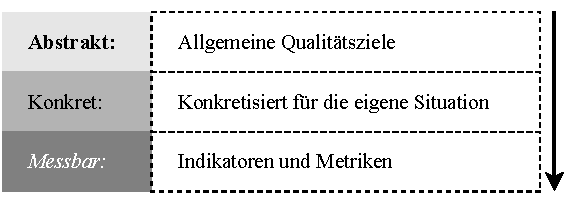
\includegraphics{contents/02_basics/res/quality_models.pdf}
    \caption{Aufbau eines Qualitätsmodells in drei Ebenen \cite[S. 34, ][]{schneider2012abenteuer}}
    \label{fig:basics_quality_models}
\end{figure}

\cite{schneider2012abenteuer}